\documentclass[12pt,twoside]{article}
%%%%%%%%%%%%%%%%%%%%%%%%%%%%%%%%%%%%%%%%%%%%%%%%%%%%%%%%%%%%%
% Languages:

% Falls die Ausarbeitung in Deutsch erfolgt:
\usepackage[ngerman]{babel}
\usepackage[T1]{fontenc}
\renewcommand*\rmdefault{cmr}
% \usepackage[latin1]{inputenc}
% \usepackage[latin9]{inputenc}
\usepackage[utf8]{inputenc}
\selectlanguage{ngerman}

% If the thesis is written in English:
% \usepackage[english]{babel} 						
% \selectlanguage{english}

%%%%%%%%%%%%%%%%%%%%%%%%%%%%%%%%%%%%%%%%%%%%%%%%%%%%%%%%%%%%%
% Meta informations:

\newcommand{\trauthor}{Louis Kobras, Utz Pöhlmann}
\newcommand{\trtype} {Praktikumsbericht} %{Seminar Paper} %{Seminararbeit}
\newcommand{\trcourse}{\phantom{}\hspace{1.6cm}Sofrwareentwicklungspraktikum
\newline Agile Softwareentwicklung}
\newcommand{\trtitle}{Ein KUULer Praktikumsbericht} % {Verfahren in aktuellen Sprach\"ubersetzungssystemen}
\newcommand{\trmatrikelnummer}{6658699, 6663579}
\newcommand{\tremail}{4kobras@informatik.uni-hamburg.de, 4poehlma@informatik.uni-hamburg.de}
\newcommand{\trarbeitsbereich}{Students, SSE}
\newcommand{\trdate}{\today}


%%%%%%%%%%%%%%%%%%%%%%%%%%%%%%%%%%%%%%%%%%%%%%%%%%%%%%%%%%%%%
% Bind packages:
\usepackage{acronym}                    % Acronyms
\usepackage{algorithmic}								% Algorithms and Pseudocode
\usepackage{algorithm}									% Algorithms and Pseudocode
\usepackage{amsfonts}                   % AMS Math Packet (Fonts)
\usepackage{amsmath}                    % AMS Math Packet
\usepackage{amssymb}                    % Additional mathematical symbols
\usepackage{amsthm}
\usepackage{booktabs}                   % Nicer tables
%\usepackage[font=small,labelfont=bf]{caption} % Numbered captions for figures
\usepackage{color}                      % Enables defining of colors via \definecolor
\definecolor{uhhRed}{RGB}{254,0,0}		  % Official Uni Hamburg Red
\definecolor{uhhGrey}{RGB}{122,122,120} % Official Uni Hamburg Grey
% custom colors
\definecolor{pblue}{rgb}{0.13,0.13,1}
\definecolor{pgreen}{rgb}{0,0.5,0}
\usepackage{fancybox}                   % Gleichungen einrahmen
\usepackage{fancyhdr}										% Packet for nicer headers
%\usepackage{fancyheadings}             % Nicer numbering of headlines

%\usepackage[outer=3.35cm]{geometry} 	  % Type area (size, margins...) !!!Release version
%\usepackage[outer=2.5cm]{geometry} 		% Type area (size, margins...) !!!Print version
%\usepackage{geometry} 									% Type area (size, margins...) !!!Proofread version
\usepackage[outer=3.15cm]{geometry} 	  % Type area (size, margins...) !!!Draft version
\geometry{a4paper,body={5.8in,9in}}

\usepackage{graphicx}                   % Inclusion of graphics
%\usepackage{latexsym}                  % Special symbols
\usepackage{longtable}									% Allow tables over several parges
\usepackage{listings}                   % Nicer source code listings
\usepackage{multicol}										% Content of a table over several columns
\usepackage{multirow}										% Content of a table over several rows
\usepackage{rotating}										% Alows to rotate text and objects
\usepackage[hang]{subfigure}            % Allows to use multiple (partial) figures in a fig
%\usepackage[font=footnotesize,labelfont=rm]{subfig}	% Pictures in a floating environment
\usepackage{tabularx}										% Tables with fixed width but variable rows
\usepackage{url,xspace,boxedminipage}   % Accurate display of URLs
\usepackage{perpage}					% make something that is usually document-wide per page
\MakePerPage{footnote}					% make footnotes count per page instead of per document
% code snippets
\usepackage{listings}
% listing captions
\usepackage{caption}


%%%%%%%%%%%%%%%%%%%%%%%%%%%%%%%%%%%%%%%%%%%%%%%%%%%%%%%%%%%%%
% Configurationen:

\hyphenation{whe-ther} 									% Manually use: "\-" in a word: Staats\-ver\-trag

%\lstloadlanguages{C}                   % Set the default language for listings
\DeclareGraphicsExtensions{.pdf,.svg,.jpg,.png,.eps,.jpeg} % first try pdf, then eps, png and jpg
\graphicspath{{img/}} 								% Path to a folder where all pictures are located
\pagestyle{fancy} 											% Use nicer header and footer

% Redefine the environments for floating objects:
\setcounter{topnumber}{3}
\setcounter{bottomnumber}{2}
\setcounter{totalnumber}{4}
\renewcommand{\topfraction}{0.9} 			  %Standard: 0.7
\renewcommand{\bottomfraction}{0.5}		  %Standard: 0.3
\renewcommand{\textfraction}{0.1}		  	%Standard: 0.2
\renewcommand{\floatpagefraction}{0.8} 	%Standard: 0.5

% Tables with a nicer padding:
\renewcommand{\arraystretch}{1.2}

%%%%%%%%%%%%%%%%%%%%%%%%%%%%
% Additional 'theorem' and 'definition' blocks:
\theoremstyle{plain}
% \newtheorem{theorem}{Theorem}[section]
\newtheorem{theorem}{Satz}[section]		% Wenn in Deutsch geschrieben wird.
% \newtheorem{axiom}{Axiom}[section] 	
\newtheorem{axiom}{Fakt}[section]			% Wenn in Deutsch geschrieben wird.
%Usage:%\begin{axiom}[optional description]%Main part%\end{fakt}

\theoremstyle{definition}
\newtheorem{definition}{Definition}[section]

%Additional types of axioms:
\newtheorem{lemma}[axiom]{Lemma}
\newtheorem{observation}[axiom]{Observation}

%Additional types of definitions:
\theoremstyle{remark}
\newtheorem{remark}[definition]{Bemerkung} % Wenn in Deutsch geschrieben wird.
% \newtheorem{remark}[definition]{Remark} 

%%%%%%%%%%%%%%%%%%%%%%%%%%%%
% Provides TODOs within the margin:
\newcommand{\TODO}[1]{\marginpar{\emph{\small{{\bf TODO: } #1}}}}

%%%%%%%%%%%%%%%%%%%%%%%%%%%%
% Abbreviations and mathematical symbols
\newcommand{\modd}{\text{ mod }}
\newcommand{\RS}{\mathbb{R}}
\newcommand{\NS}{\mathbb{N}}
\newcommand{\ZS}{\mathbb{Z}}
\newcommand{\dnormal}{\mathit{N}}
\newcommand{\duniform}{\mathit{U}}

\newcommand{\erdos}{Erd\H{o}s}
\newcommand{\renyi}{-R\'{e}nyi}

% parameter definition for lstlistings
\lstset{ %
language=Java,   							% choose the language of the code
basicstyle=\small\ttfamily,  				% the size of the fonts that are used for the code
numbers=left,                   			% where to put the line-numbers
numbersep=5pt,                  			% how far the line-numbers are from the code
backgroundcolor=\color{light-light-gray},   % choose the background color. You must add
frame=lrtb,           						% adds a frame around the code
tabsize=4,          						% sets default tabsize to 2 spaces
captionpos=b,           					% sets the caption-position to bottom
breaklines=true,        					% sets automatic line breaking
xleftmargin=0.5cm,							% space from the left paper edge
commentstyle=\color{pgreen},
keywordstyle=\color{pblue},
literate=%
    {Ö}{{\"O}}1
    {Ä}{{\"A}}1
    {Ü}{{\"U}}1
    {ß}{{\ss}}1
    {ü}{{\"u}}1
    {ä}{{\"a}}1
    {ö}{{\"o}}1
    {~}{{\textasciitilde}}1
}
\renewcommand{\lstlistingname}{Code}
\captionsetup[lstlisting]{font={footnotesize},margin=1.5cm,singlelinecheck=false } % removes "Listing 1: "
\definecolor{light-light-gray}{gray}{0.95}


%%%%%%%%%%%%%%%%%%%%%%%%%%%%%%%%%%%%%%%%%%%%%%%%%%%%%%%%%%%%%
% Document:
\begin{document}
\setlength{\headheight}{14.5pt}

\fancyhead{}
\fancyhead[LE]{ \slshape \trauthor}
\fancyhead[LO]{}
\fancyhead[RE]{}
\fancyhead[RO]{ \slshape \trtitle}

%%%%%%%%%%%%%%%%%%%%%%%%%%%%
% Cover Header:
\begin{titlepage}
	\begin{flushleft}
		Universit\"at Hamburg\\
		Department Informatik\\
		\trarbeitsbereich\\
	\end{flushleft}
	\vspace{3.5cm}
	\begin{center}
		\huge \trtitle\\
	\end{center}
	\vspace{3.5cm}
	\begin{center}
		\normalsize\trtype\\
		[0.2cm]
		\Large\trcourse\\
		[1.5cm]
		\Large \trauthor\\
		[0.2cm]
		\normalsize Matr.Nr. \trmatrikelnummer\\
		[0.2cm]
		\normalsize\tremail\\
		[1.5cm]
		\Large \trdate
	\end{center}
	\vfill
\end{titlepage}

	%backsite of cover sheet is empty!
\thispagestyle{empty}
\hspace{1cm}
\newpage

%%%%%%%%%%%%%%%%%%%%%%%%%%%%
% Lists:
\setcounter{tocdepth}{2} 					% depth of the table of contents (for Seminars 2 is recommented)
\tableofcontents
\pagenumbering{arabic}
\clearpage

%%%%%%%%%%%%%%%%%%%%%%%%%%%%
% Content:

% the actual content, usually separated over a number of sections
% each section is assigned a label, in order to be able to put a
% crossreference to it

\section{Einleitung}
\label{sec:intro}
%%%%%%%%%%%%%%%%%%%%%%%%%%%%%%%%%%%%%%%%%%%%%%%%%%%%%%%%%%%%%%%%%%%%%%%
%Es war einmal ein Spiel namens \textit{Zuul}.
%\textit{Zuul} war ein neues, unglaublich langweiliges Spiel.
%Doch dann begann \dots das Praktikum!\\
%Ein kleines Team unerfahrener Entwickler bekam den Auftrag, aus \textit{Zuul} etwas zu machen.
%Anhand von Kundenwünschen und mit Einspeisen eigener Ideen wurde aus \textit{Zuul} letztendlich ein neues, unglaublich geiles Spiel.\\
%Sein Name ist... \textbf{KUUL}.\\
%\\
%\textit{KUUL} ist ein recht simples Adventure-Spiel mit Unterstützung von Maus- und Tastatursteuerung.
%Das Story-Konzept ist, dass der Spieler in einem Raum aufwacht und entweder durch Finden eines bestimmten Gegenstandes oder durch erfolgreiches Verlassen der Karte das Spiel gewinnt, wobei zum Verlassen der Karte ein anderer bestimmter Gegenstand erforderlich ist.\\
%Anhand der Basis von \textit{Zuul} wurde die erste Welt soweit erweitert, dass es sich um einen Universitäts-Campus handelt, während die zweite Welt nach Kundenwunsch an den Hamburger Kiez angelehnt ist.
%\section{Hauptteil}
%\label{sec:main}
%
%\subsection{Einleitung}
%Es begab sich aber zu der Zeit des Softwareentwicklungspraktikums, als ein unglaublich langweiliges Spiel noch neu war, dass eine Gruppe junger, unerfahrener, patriotischer Softwareentwickler in spe sich an die schwierige, überwältigende, kaum lösbare Aufgabe wagte, diesem Spiel Leben einzuhauchen.\\
%\subsection{Hauptteil}
%Sie haben es geschafft.\\
%\subsection{Schluss}
%Und wenn sie nicht gestorben sind, programmieren sie noch heute!
%\-\\
%\-\\
%%%%%%%%%%%%%%%%%%%%%%%%%%%%%%%%%%%%%%%%%%%%%%%%%%%%%%%%%%%%%%%%%%%%%%%
Dieser Bericht befasst sich mit dem Praktikum Agile Softwareentwicklung\footnote{STiNE-Veranstaltungsnummer 64-142} (im Folgenden \"ASE") als Teil des Moduls Softwareentwicklungspraktikum\footnote{STiNE-Modulnummer SSE\_PR} (im Folgenden \string"SEP"), absolviert im zweiten Fachsemester (im Folgenden "FS2") des Studiengangs Software-System-Entwicklung (im Folgenden \string"SSE").\\
Dieser Bericht ist geschrieben aus Sicht der Teilnehmer des Teilkurses 3 (ASE-SEP3), in welchem das Zuul-Ausgangssystem, welches von den Praktikumsbetreuern bereit gestellt wurde, in ein \textit{Point\& Click}-ähnliches \textit{Adventure-Game} weiterentwickelt wurde, welches nun den Titel \textit{KUUL} trägt.\\
In diesem Bericht wird tiefergehend auf die Implementation von interaktiven Objekten in das \textit{KUUL}-System eingegangen.
Dies umfasst die Erstellung der Gegenstände, deren Speicherung und die Implementation der Interaktion.
\section{Hauptteil}
\label{sec:main}
Wie bereits in der Einleitung angesprochen, wird sich dieser Bericht primär mit dem Umgang mit den Gegenständen in \textit{KUUL} befassen.
Interaktiv sind diese Gegenstände insofern, als dass sie aufgesammelt, benutzt und kombiniert werden können.\\
Zunächst wird jedoch festgestellt werden, worum es sich bei \textit{KUUL} handelt.
\subsection{KUUL}
\label{ssec:main_kuul}
\textit{KUUL} ist ein Ausbau des von den Praktikumsbetreuern bereitgestellten Zuul-Ausgangssystems.
Während Zuul ein konsolenbasiertes Text-Adventure ist, wird \textit{KUUL} mit Maus und Tastatur gesteuert.
Dies geschieht insofern, als dass Gegenstände, \textit{NPCs}\footnote{\textit{Non-Player-Character}, eine Figur im Spiel, die nicht vom Spieler, sondern vom Spiel kontrolliert wird.} und Türen angeklickt werden können, um mit ihnen zu interagieren.
Mithilfe der Tastatur kann der \textit{PC}\footnote{\textit{Player-Character}, vgl. \textit{NPC}} durch die Räume in der Welt von \textit{KUUL} bewegt werden, ebenso lassen sich alle Funktionen des Spiels über bestimmte Tasten direkt ansteuern.\\
Zuul hatte bereits einige wenige Räume vorzuweisen, die durch die Namensgebung erkennen ließen, dass es sich um eine an ein Universitätsgelände angelehnte Welt handelte.
Dies wurde vom Entwicklerteam aufgegriffen, sodass, während die Anzahl der Räume mehr als verdoppelt wurde, die Umgebung \textit{Universität} beibehalten wurde.
Auf Wunsch des Kunden hin wurde im Lauf des Praktikums eine weitere Welt hinzugefügt, die sich grob am Hamburger Kiez (im Folgenden "Kiez") orientiert.
\subsection{Entwicklungspozess}
\label{ssec:main_dev}
Da zunächst nur die Textwelt von Zuul zur Verfügung stand, wurden die ersten Gegenstände inklusive des provisorischen Gewinngegenstandes\footnote{In \textit{KUUL}, ist es auf zwei Arten möglich, zu gewinnen: Entweder findet der Spieler einen Schlüsselgegenstand, mit dem er einen Raum betreten kann, der als \textit{Siegraum} betitelt wurde, oder er findet einen \textit{Sieggegenstand}} \textit{Handy} in den Räumen platziert, die nach der Erweiterung vorhanden waren.
Auf Kundenwunsch wurde das Handy als Sieggegenstand recht schnell von der \textit{Goldananas} abgelöst.
\begin{lstlisting}[caption=Auszug aus dem XML-Parser für Gegenstände, label=code:main_parser]
if (gegenstandElement.getElementsByTagName("beenden").getLength() != 0)
{
	Node beendenNode = gegenstandElement.getElementsByTagName(
			"beenden").item(0);
	String nachricht = beendenNode.getTextContent();
	_beendenCommandListe.put(id, nachricht);
}
\end{lstlisting}
Der hier betrachtete Quellcode ist aus dem in \textit{KUUL} verwendeten XML-Parser entnommen.\\
Die XML\footnote{\textit{eXtensible Markup Language}, findet Verwendung in der Strukturierung von Daten}-Sprache arbeitet insofern, als dass jedes Dokument eine Reihe von Elementen hat, und diese Elemente haben Attribute (im Folgenden "Tags"), welche wiederum Element-Reihen seien können.
Im Gegensatz zu HTML\footnote{\textit{HyperText Markup Language}, findet Gebrauch bei der Gestaltung von Web-Oberflächen} ist XML erweiterbar, das heißt es können benutzerdefinierte Tags hinzugefügt werden; die Syntax der beiden Sprachen ist nahezu gleich.\\
An dieser Stelle wird der Tag des Gegenstands mit der Bezeichnung "beenden\" abgefragt: Ist sie vorhanden (Länge ungleich 0), so handelt es sich um einen Sieggegenstand.
Anzumerken ist hierbei, dass der verwendete Parser abgefragte Tags immer als eine Form von Liste zurückgibt, weswegen der Tag mit \texttt{.item(0);} abgefragt werden muss.\\
Die Siegnachricht, welche ebenfalls extern in der XML-Datei gelagert wird, wird ausgelesen und als String gespeichert.
Der Gegenstand wird als Tupel aus ID und der Siegnachricht in eine Liste gelegt, die an anderen Stellen im Programm aufgerufen werden kann, um festzustellen, ob der gerade verwendete Gegenstand ein Sieggegenstand war.\\
Wird der Sieggegenstand nun innerhalb des Spiels gefunden, aufgehoben und benutzt, so wird das Spiel beendet und es erscheint ein Popup, welches einen darüber informiert, dass man gewonnen hat, und den String \texttt{nachricht} (vgl. Code 1 l.5) anzeigt.
Die beiden Welten haben unterschiedliche Sieggegenstände, sodass es auf dem Kiez erforderlich ist, das eigene Portmonnaie wiederzufinden.
\subsection{Funktionsumfang}
\label{ssec:main_func}
Wie bereits mehrfach angesprochen, können Gegenstände aufgehoben und genutzt werden.\\
In \textit{Zuul} funktionierte dies über die Konsolenbefehle.
Um \textit{KUUL} komfortabler zu machen, sind Gegenstände im Raum anklickbar.
Ebenso können sie aufgehoben werden, wenn sich der Spieler direkt davor stellt und die Enter-Taste drückt.\\
Aufgenommene Gegenstände kommen in den \textit{Rucksack}, welcher allerdings nur eine beschränkte Kapazität von vier beliebigen Gegenständen hat.
Gegenstände, die man im Rucksack hat, können kombiniert werden.
Allerdings müssen sie dazu in der XML-Datei den Tag "kombinierbar", welcher im Parser als \texttt{boolean} ausgelesen wird, gesetzt bekommen.
Ist dieser Tag auf den Wert \texttt{"false"} gesetzt, so können die Gegenstände nicht kombiniert werden.\\
Eine weitere Besonderheit des Rucksack ist es, dass die meisten Gegenstände in der ersten Welt, die einem normalerweise Energie zurückgeben\footnote{Energie wird benötigt, um sich zu bewegen. Der Spieler startet mit 15 Energie-Einheiten. Jeder Raumwechsel verbraucht eine Einheit.}, mit der Zeit verfallen.
Dies führt dazu, dass sie irgendwann nicht nur keine Energie zurückgeben, sondern Energie abziehen.\\
Illustriert wird dies erstens durch eine Veränderung des Aussehens des Gegenstandes und zweitens durch eine Änderung des Textes, der bei Nutzung des Gegenstandes angezeigt wird\footnote{So wird z.B. \textit{"Die Ananas stärkt Sie und gibt Ihnen Kraft. Sie erhalten 2 Lebenspunkte. Toll!"} zu \textit{"Die Ananas ist bis auf den Kern vergammelt. Sie verlieren Lebenspunkte!"}, wenn man die Ananas lange genug im Rucksack behält}.
Graphisch hat jeder Gegenstand höchstens drei Phasen\footnote{Viele Gegenstände, wie zum Beispiel Schlüssel, haben nur eine Phase}, der Abzug der Energie-Einheiten wächst allerdings stetig linear.
Alle zwei Schritte zieht der Gebrauch eines solchen Gegenstandes eine Einheit mehr ab.
\begin{lstlisting}[caption=Teilimplementation der Verringerung der Energieregeneration, label=code:main_func]
if (_verfallszeitpunkt > 1) {
	_verfallszeitpunkt = 0;
	lebensCommand.verringereLebenspunkte();
	if (lebensCommand.getLebensEffekt() == 0) {
		setIcon("Graphics/Items/Phase2" + "/" + gibName() + "2.png");
		_verfallStatus = 1;
		return true;
	} else if (lebensCommand.getLebensEffekt() < 0) {
		setIcon("Graphics/Items/Phase3" + "/" + gibName() + "3.png");
		_verfallStatus = 2;
		return true;
	}
} else {
	_verfallszeitpunkt++;
}
\end{lstlisting}
Bei dem Feld \texttt{\_verfallszeitpunkt}\footnote{Nomenklaturregeln nach SE2-Format} handelt es sich um eine Exemplarvariable vom Typ Integer.
Immer dann, wenn der hier gezeigte Block aufgerufen wird, wird diese Variable geprüft.
Ist sie auf 0, wird sie inkrementiert; ist sie auf 1, so wird der Effekt des Lebenskommandos\footnote{interne Umsetzung der Energieverwaltung, für die Verwendung der Gegenstände nicht weiter von Bedeutung} dekrementiert und der \texttt{\_verfallszeitpunkt} wird wieder auf 0 gesetzt.
Was ebenfalls zu sehen ist, ist, dass ein neues Icon für den Gegenstand gesetzt wird, wenn er 0 Energie-Einheiten erreicht beziehungsweise sobald er anfängt, Energie abzuziehen (siehe den inneren if-Block).\\
\\
Zur bereits angesprochenen Kombinationsfunktion sei gesagt, dass nicht alle Gegenstände kombinierbar sind.
Es wurde bereits gesagt, dass ein Tag gesetzt werden muss, damit ein Gegenstand vom \textit{Crafting Tool} (vgl. Abb. \ref{fig:main_craft}) akzeptiert wird.
Desweiteren muss es ein Rezept geben, welches den fraglichen Gegenstand beinhält.
Befindet sich dann der zweite Gegenstand ebenfalls im Rucksack des Spielers, so kann der Spieler die Kombination ausführen.\\
Da sich die zweite Welt an den Kiez anlehnt, befinden sich dort primär alkoholische Getränke.
Alle alkoholischen Getränke können miteinander kombiniert werden; allerdings ist dort die Regelung ein wenig anders: Jedes Rezept hat als Ergebnis eine \textit{Gute Mische}, welche Energie dazu gibt, jedes ungültige Rezept hat als Ergebnis eine \textit{Schlechte Mische}, welche Energie abzieht.
\begin{figure}[h!bt]
    \begin{center}
        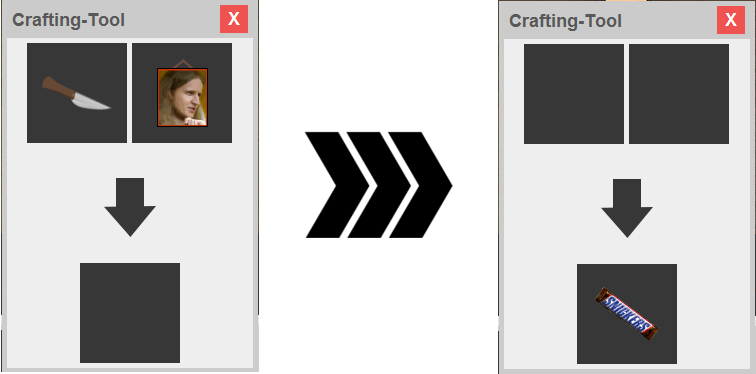
\includegraphics[width=0.35\textwidth]{img/craftingUI.png}
        \label{fig:main_craft}
    	\caption{Crafting Tool}
    \end{center}
\end{figure}
Die hier betrachtete Konfiguration des \textit{Crafting Tools} entstammt der ersten Welt.
Das Messer und das Gemälde werden kombiniert, um ein Snickers zu erhalten, welches die Energie vollständig wieder auffüllt.
Messer und Gemälde werden dabei verbraucht.
\subsection{Inhaltliches}
\label{ssec:main_cont}


\section{Schluss}
\label{sec:end}

\end{document}


